\chapter{Looking for Supercoiling Epistasis in \emph{EvoTSC}}
\label{chap:epistasis}

The results obtained with the \emph{EvoTSC} model that I have presented up until now tackle the role that DNA supercoiling plays in the evolution of the structure of bacterial genomes, via the transcription-supercoiling coupling.
In this chapter, I take the \emph{EvoTSC} model in another direction, in order to return to the idea of epistasis between mutations in the supercoiling level and other mutations that was the root question of the research agenda of my PhD.
In the experiment conducted with \emph{Aevol} and presented in Chapter~\ref{chap:aevol}, the main hypothesis to explain why I was not able to detect a signal of epistasis between supercoiling mutations and other kinds of mutations is that the model of supercoiling that I implemented could be too restricted.
As a result, supercoiling mutations in that model would not generate interesting enough evolutionary paths to explore the fitness landscape in a qualitatively different way than in their absence.
In \emph{EvoTSC}, supercoiling is on the contrary sufficiently finely modeled to allow the evolution of regulatory networks based on local variations in the level of supercoiling, as demonstrated in the previous chapters.

In this chapter, I therefore present an experiment, inspired by the \emph{LTEE}, in which previously evolved individuals must adapt to a new environment.
In order to conduct this experiment in the \emph{EvoTSC} model, I introduced a little change to the model, by letting the supercoiling level of individuals evolve, as in the experiment using \emph{Aevol} presented in Chapter~\ref{chap:aevol}.
However, unlike in the \emph{Aevol} experiment, the non-linear effect of the basal supercoiling level on gene expression in the \emph{EvoTSC} model could this time allow populations in which supercoiling evolves to follow qualitatively different evolutionary trajectories than populations with a constant supercoiling level.
I first present the methodology of this new experiment, including  the new mutational operator for the supercoiling level.
Then, I compare the evolution of populations with and without supercoiling mutations in a new environment.
Finally, I investigate more thoroughly the fitness landscapes that are explored by the supercoiling mutations.


\section{Experimental Framework}

Performing exactly the same experiment as the one in \emph{Aevol} described in Chapter~\ref{chap:aevol} is not possible in \emph{EvoTSC} (at the time of writing), as the ancestry tree of the population throughout generations and the precise set of mutations at each reproduction event are not recorded.
Studying the lineage of the final population in order to study the properties of the mutations that fixed in the lineage is therefore not possible in \emph{EvoTSC}.
I therefore devised another experiment, which reproduces the setup of the \emph{LTEE} in an \emph{in silico} setting, in order to evaluate the possible epistatic interactions between supercoiling mutations and other mutations.

The experiment consists in two successive sets of evolutionary runs.
The initial set consists in the evolution of two groups of populations, with and without supercoiling mutations, for 1,000,000 generations, from which to extract \emph{wild-type} (evolved) individuals.
In order to model the change of environment from the \emph{LTEE} in the \emph{EvoTSC} model, I reassign arbitrary types to every gene in the genome of the wild-type individuals, but keep the number of genes of each type constant, individuals.
As the environment in \emph{EvoTSC} is represented by a pair of environments (A and B) with different expression targets, this corresponds to replacing these environments with new environments A' and B', in which new subsets of genes must be activated or inhibited.
We call this change of environment an \emph{environmental shock}, and the individuals with shuffled gene types \emph{shocked} individuals.
I then used these shocked individuals to create new populations, and let these populations evolve in the new environments to study their re-adaptation.

\subsection{Introducing Supercoiling Mutations}

The mutational operator that I used for the mutations in the basal supercoiling level $\sigma_{basal}$ of individuals in \emph{EvoTSC} is similar to the one I implemented in \emph{Aevol} and that is presented in Section~\ref{sec:aevol:mut-sc}.
When mutating an individual, we first decide whether to mutate its basal supercoiling level with a probability $p$, and draw a small change $\delta\sigma_{basal}$ to be added to the supercoiling level according to a normal law $\mathcal{N}(0, s^2)$.
In this experiment, $p=0.1$ and $s^2=0.0001$.
Then, exactly as in the main experiment, the individual can undergo a series of genomic inversions which rearrange the relative position of genes on their genome.

\begin{figure}
\centering
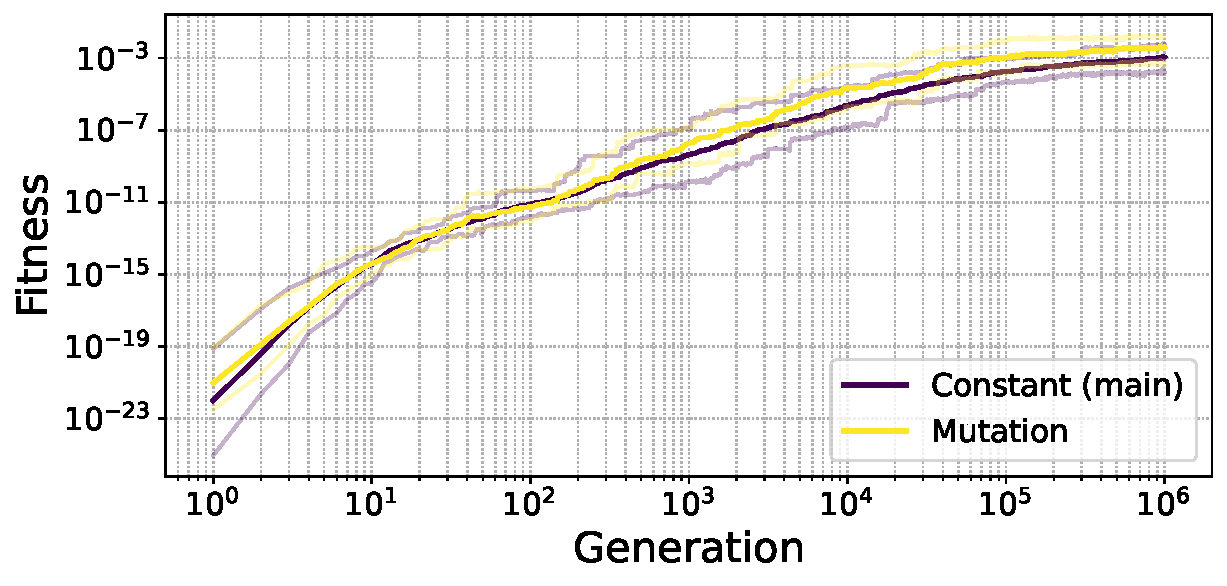
\includegraphics[width=0.8\textwidth]{epistasis/img/fitness_all_with_main.pdf}
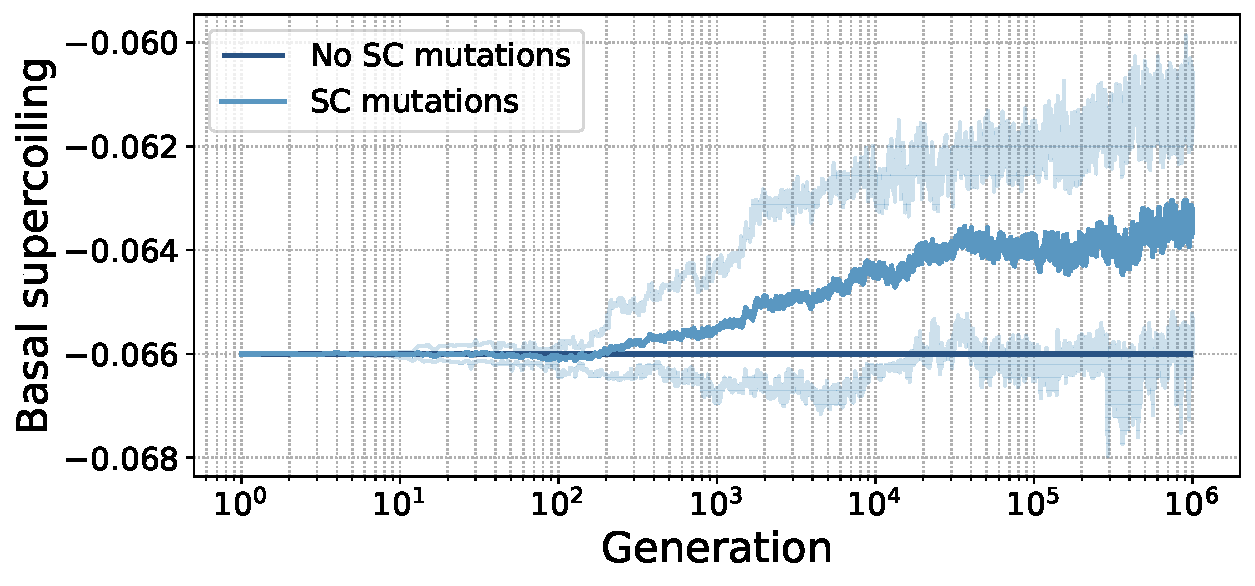
\includegraphics[width=0.8\textwidth]{epistasis/img/basal_sc_all.pdf}
\caption[Average basal supercoiling and fitness during evolution of the wild-types, with basal supercoiling level mutations]{Top: average fitness of the best individual in every replicate during evolution, for the 10 wild-types with (light blue) and the 30 wild-types without (dark blue) supercoiling mutations.
Bottom: average basal supercoiling level of the best individual in every replicate during evolution of the wild-types with (light blue) and without (dark blue) supercoiling mutations.
Lighter lines represent the first and last decile of the data.}
\label{fig:epistasis:wt-evolution}
\end{figure}

Figure~\ref{fig:epistasis:wt-evolution} presents the evolution of the fitness (top) and basal supercoiling level (bottom) of the best individual in each replicate during the evolution of the wild-type populations, with and without supercoiling mutations.
We can first see that, in the wild-types that evolve with supercoiling mutations (light blue), fitness evolves in a qualitatively similar fashion to the main run, and appears to be slightly higher by the end of evolution than without supercoiling mutations.
Then, looking at the basal supercoiling level, we can see that the average level of negative supercoiling decreases over time during evolution.
This indicates that the supercoiling level can indeed be targeted by selection in the model, and that there is furthermore a clear selection pressure towards reducing the amount of negative supercoiling.
A possible hypothesis to explain both the higher fitness and lower negative supercoiling level of wild-types with supercoiling mutations comes from recalling that, with the initial basal supercoiling level of $\sigma_{basal} = -0.066$, genes tend to have a high expression level in both environments (see the dash-dotted curve of Figure~\ref{fig:ploscb:activity-by-sigma}).
As a consequence, decreasing the level of negative supercoiling of the genome corresponds to shifting the background supercoiling in both environments to a less negative value.
This lessens the bias towards high gene expression in both environments, and therefore helps the inhibition of \emph{A} genes in environment B in these populations (data not shown).

\subsection{Environmental Shock}

\begin{figure}
\centering
\begin{elasticrow}[width=\textwidth]
\elasticfigure{epistasis/img/init_indiv_wt_00_no_shuffle_env_A.pdf}
\elasticfigure{epistasis/img/init_indiv_wt_00_shuffle_00_env_A.pdf}
\end{elasticrow}
\caption[Evolved wild-type individual before and after an environmental shock]{Genome of one of the wild-types that evolved with supercoiling mutations (left), and shocked individual created from that individual (right), both evaluated in environment A.
The gene type (color) and activity (light or dark) of two-thirds of the genes changes, but not the local supercoiling level, as relative gene positions and gene expression levels remain constant.}
\label{fig:epistasis:shock}
\end{figure}

In order to simulate the effect of an environmental shock on a given individual, that is to say replacing environments A and B by new environments A' and B', we assign a new type at random to every gene on the genome of this individual, ensuring that the number of genes of each type remains constant.
As there are 3 gene types (\emph{A}, \emph{B}, and \emph{AB}), each gene has one in three chances of actually staying of the same type, and two in three chances of actually changing types.
This represents the fact that some genes that had to be activated (resp. inhibited) in environment A or B must now be inhibited (resp. activated) in environment A' or B'.
Note that the only thing that changes is the genes that must be activated in each environment, but not the shift in supercoiling caused by either environment.

A representative example of an environmental shock is depicted in Figure~\ref{fig:epistasis:shock}.
On the left-hand side is the genome of a wild-type individual that evolved with supercoiling mutations, and on the right-hand side is the result of applying an environmental shock to this individual.
The type (color) of two third of the genes changes, but not the local supercoiling level along the genome, as the gene positions themselves -- and hence their expression level, as determined by the transcription-supercoiling coupling -- remain unchanged.
As a result, a large number of genes end up wrongly activated or inhibited, which opens the door to future compensatory mutations in the adaptation to this new environment.

\subsection{Experimental Protocol}

The populations that I used for the wild-types without supercoiling mutations are the main populations already presented in detail in Chapters~\ref{chap:ploscb} and~\ref{chap:param}.
For the wild-types with supercoiling mutations, I evolved 10 new populations, for the same number of generations (1,000,000) as the main runs, with all other parameters kept exactly the same.
I then chose 5 representative wild-types at random from each set of simulations.
From each of these wild-type individuals that evolved with or without supercoiling mutations, I created 5 different individuals with shuffled genes representing the effect of an environmental shock as described above, resulting in 25 shocked individuals in total.
For each shocked individual, I then created 5 populations, each initialized with clones of that individual but with different seeds, and let each population evolve for 250,000 generations, in order to recover from the environmental shock.
This allowed me to compare the speed of evolution after an environmental shock in 125 populations with, and 125 populations without, mutations in the basal supercoiling level.


\section{Evolution after an Environmental Shock}

\begin{figure}[H]
\centering
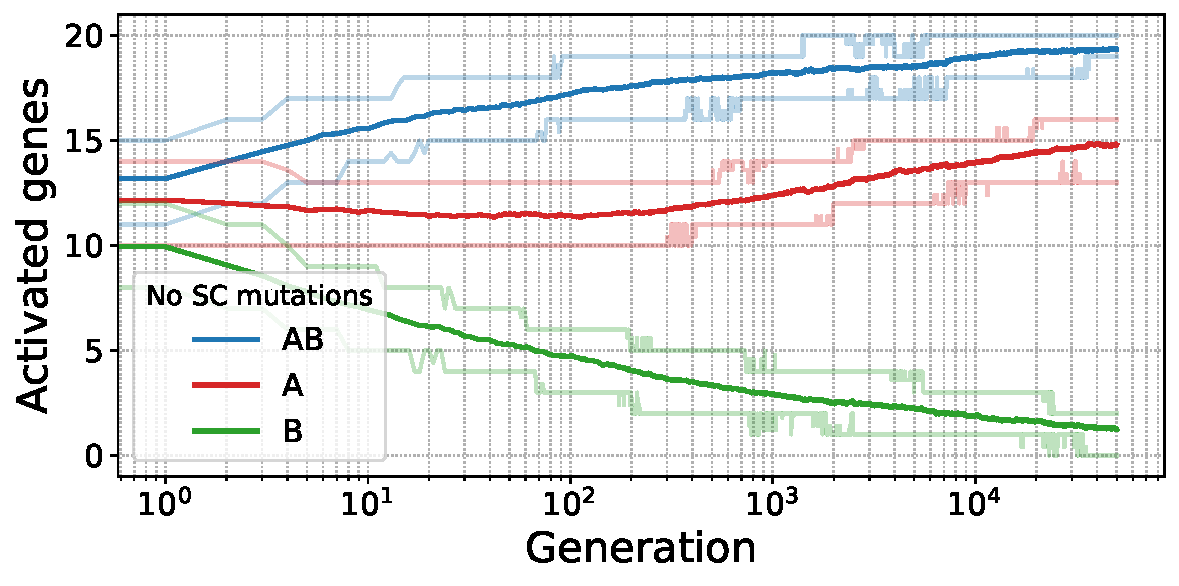
\includegraphics[width=0.495\textwidth]{epistasis/img/control/gene_activity_env_A.pdf}
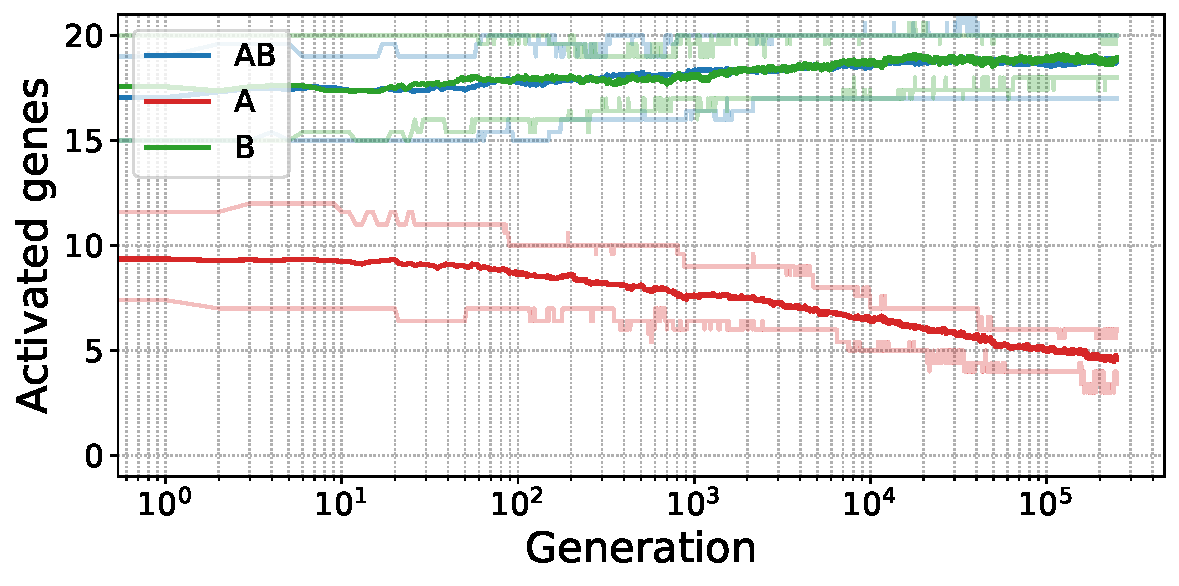
\includegraphics[width=0.495\textwidth]{epistasis/img/control/gene_activity_env_B.pdf}

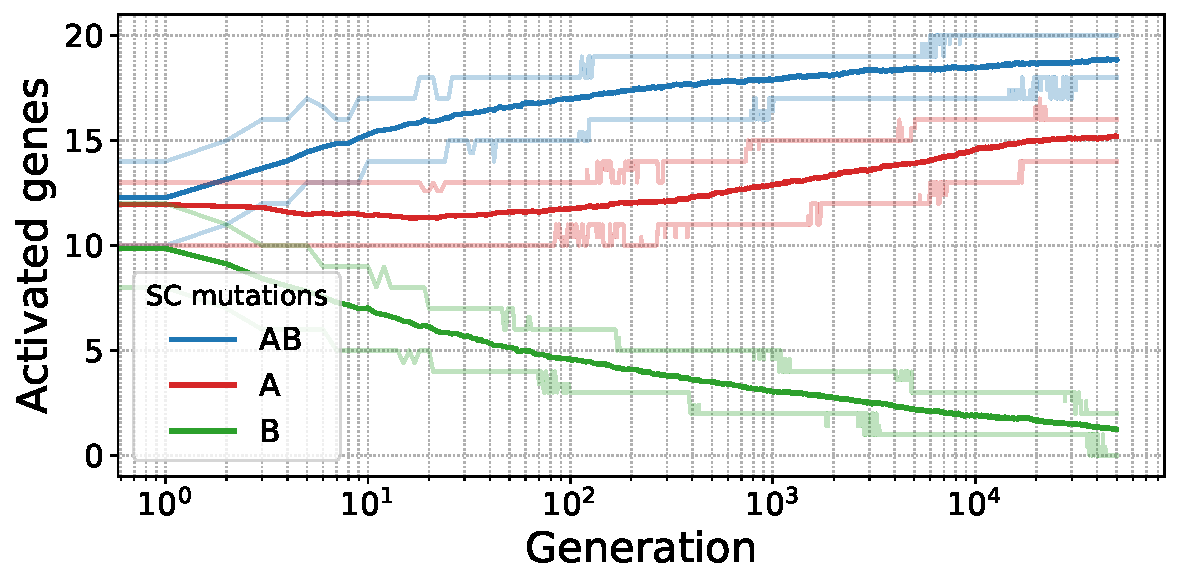
\includegraphics[width=0.495\textwidth]{epistasis/img/with-sc/gene_activity_env_A.pdf}
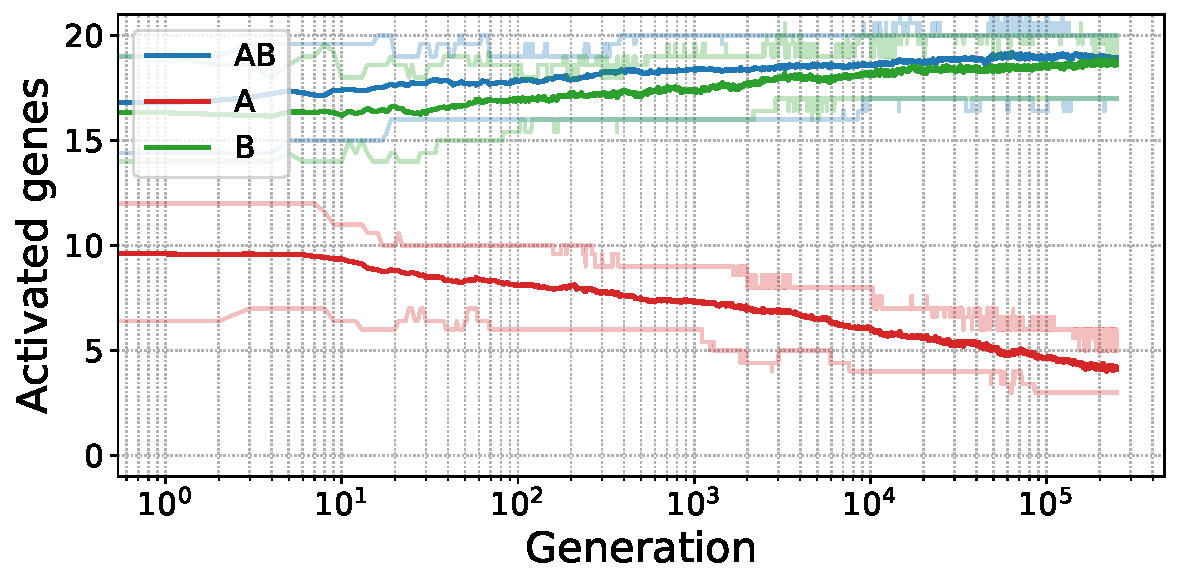
\includegraphics[width=0.495\textwidth]{epistasis/img/with-sc/gene_activity_env_B.pdf}
\caption[Evolution of the number of activated genes in each environment, with a]{Average number of activated genes of each type in environment A (left) and B (right) during evolution, without (top) and with (bottom) supercoiling mutations.
Lighter lines represent the first and last decile of the data.}
\label{fig:epistasis:activ-by-env}
\end{figure}

Figure~\ref{fig:epistasis:activ-by-env} shows the evolution of the average number of activated genes by type in each environment after the environmental shocks, averaged over the 25 simulations without supercoiling level mutations (top) and the 25 simulations with supercoiling level mutations (bottom).
In both cases, the number of activated genes in each environment initially regresses towards one half as a consequence of the environmental shock, but evolves again towards their respective targets.

\begin{figure}
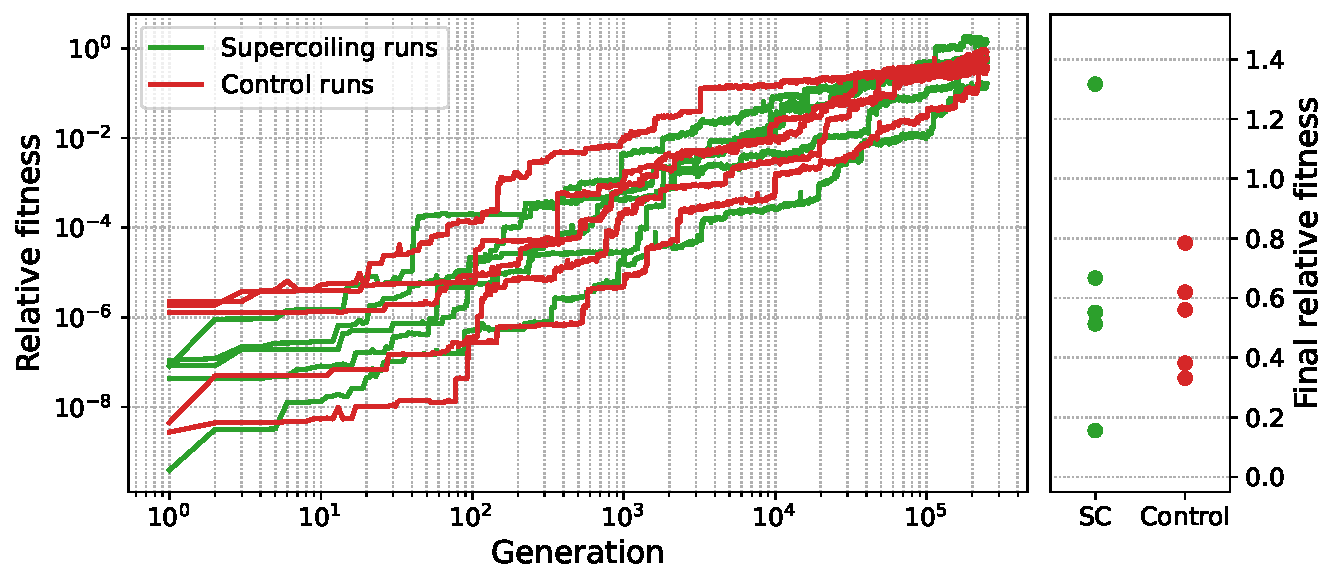
\includegraphics[width=\textwidth]{epistasis/img/rel_fitness_sc_control.pdf}
\caption[Average relative fitness to the ancestor, during evolution after an environmental shock]{Left: relative fitness of the best individual in each simulation compared to the corresponding wild-type, averaged over the 5 replicates for each wild-type, at every generation.
Right: average relative fitness of the 5 replicates for each wild-type at the end of the simulations.}
\label{fig:epistasis:rel-fitness}
\end{figure}

Recall that the point of this experiment is to detect whether populations with supercoiling mutations evolve faster than populations without, which we can interpret as a sign of positive epistasis between supercoiling mutations and other mutations.
In order to be able to compare the speed of evolution between the populations started from the different wild-types, we are therefore interested in the evolution of the fitness of each population compared to its original wild-type.
Figure~\ref{fig:epistasis:rel-fitness} shows the evolution of this relative fitness, averaged over the 5 replicates for each wild-type, both during evolution (left) and at the last generation (right), with (green) or without (red) supercoiling mutations.

Two main observations are possible on the figure.
First, all populations evolve a fitness that is on the same order of magnitude as their ancestor by 250,000 generations, showing that the environmental shock has been successfully compensated during evolution.
Second, we can observe the populations with supercoiling mutations do not seem to evolve faster than the populations without these mutations, as there is no clear separation between the relative fitness curves of each set of populations.
This lack of separation remains in particular true at the last generation of the simulations, as shown on the right-hand side of the figure: the simulations with supercoiling mutations span a broader range of relative fitness values than the simulations without.
These results therefore tend to indicate that, within the context of this experiment, introducing mutations in the basal supercoiling level does not seem to play a role in accelerating evolution, even though it does allow for a higher fitness overall.


\section{Supercoiling Fitness Landscapes}

blabliblou


\section{Discussion}

In the experiment presented in this chapter, I evaluated the speed at which populations recover their fitness after an environmental shock that changes the expression target of a subset of genes.
I compared the speed of evolution of populations in which the supercoiling basal level evolves and of populations in which it does not, by measuring the relative fitness of each population after 250,000 generations of evolution to their ancestor before the environmental shock.
I was not able to observe a statistically significant difference between the relative fitnesses of each kind of population, which could have been interpreted as a sign of positive epistasis between supercoiling mutations and genomic inversions.

This negative result can be analyzed in several ways.
First, it is of course possible for a signal to appear if I were to increase the number of wild-type individuals subjected to environmental shock, or the number of environmental shocks for each wild-type individual, in order to average out the contingent evolutionary trajectories before and after the shocks.
Given the evolutionary trajectories in Figure~\ref{fig:epistasis:rel-fitness}, this does however not seem very likely.
Second, it is also possible that by analyzing the lineages as in the \emph{Aevol} experiment presented in Chapter~\ref{chap:aevol}, a pattern in which genomic inversions fix faster after a basal supercoiling change could be detected.
Once again, the negative result of the \emph{Aevol} experiment rather diminishes the likeliness of finding such a positive signal.
Finally, the gene expression targets used in the \emph{EvoTSC} model are extremely simple, with the only targets being maximal and minimal expression.
Fitness peaks are therefore separated by extremely wide valleys in the fitness landscape, and basal supercoiling level mutations might not allow population to cross these valleys frequently enough to play a meaningful role in re-adaptation after an environmental shock.
A version of the \emph{EvoTSC} model in which gene expression targets are chosen from a continuous space, rather than a discrete set of values, would not only be more biologically realistic than the current version, but might also present a fitness landscape in which supercoiling mutations can play a more significant evolutionary role.